\section{Pruebas y resultados}\label{sec:montaje_pruebas}

Las pruebas del prototipo siguen la rama ascendente del modelo en V adoptado en el proyecto: primero se verifican los componentes y los enlaces por separado, después los subsistemas integrados y, por último, el sistema completo frente a los requisitos. Este orden permite aislar las fallas, ya que una prueba superada en un nivel inferior descarta ese elemento como causa de un error en un nivel superior. Todas las pruebas se realizan con agua y, en las fases con detergente, con una sustancia segura que lo representa, de acuerdo con las restricciones de seguridad del proyecto. A continuación se describen las pruebas ejecutadas en el segundo y el tercer corte, su relación con los requisitos y las pendientes.

\subsection{Comunicación entre el PLC y la HMI}

La primera prueba de integración fue el enlace PROFINET entre el PLC S7-1200 y la HMI KTP600 Basic, realizado desde el primer corte. Se transmitieron dos señales: la variable \texttt{CONTADOR\_HMI} (tipo INT, dirección \texttt{\%MW2}), enviada por el PLC y visualizada en la HMI, y la variable \texttt{C1\_Estado\_HMI}, vinculada a una barra gráfica que representa el estado del sistema. El intercambio de datos y su visualización en la interfaz de operador se verificaron correctamente (Tabla~\ref{tab:evidencia_comunicacion}), lo que confirmó la base de comunicación local sobre la que se construyó la operación del prototipo.

\subsection{Supervisión remota}

La API de supervisión registró 5831 lecturas hasta el 19 de octubre de 2026, que la interfaz web muestra (Sección~\ref{sec:montaje_comunicaciones}). La verificación de la cadena completa confirmó la actualización de las variables en la HMI y en la interfaz remota con un periodo de 30\,s o menos (VAL-10). El comportamiento del PLC ante la pérdida de la HMI ya se verificó en el laboratorio 4 de Comunicaciones Industriales \cite{ruiz2026lab4}.

\subsection{Ensayo de identificación térmica}

Con el tanque de mezcla lleno se ejecutó el ensayo de escalones de potencia descrito en la Sección~\ref{sec:montaje_control}. La temperatura se adquirió con el PT100 y el transmisor SITRANS: la corriente de 4--20\,mA circula por la resistencia de 500\,$\Omega$ y produce entre 2 y 10\,V en la entrada analógica de 0--10\,V del PLC, que entrega 27\,648 cuentas a 10\,V. Por tanto, el rango útil de la señal va de 5\,530 cuentas (4\,mA, 0\,°C) a 27\,648 cuentas (20\,mA, 100\,°C), límites con los que se configuraron las instrucciones \texttt{NORM\_X} y \texttt{SCALE\_X}.

El registro contiene 648 datos, uno cada 5\,s, a lo largo de 54\,min, con escalones de 0\,\% de potencia entre 0 y 2\,min, 100\,\% (2000\,W) entre 2 y 11\,min, 50\,\% (1000\,W) entre 11 y 24\,min, 100\,\% entre 24 y 34\,min y 0\,\% entre 34 y 54\,min. Durante el ensayo la temperatura del agua subió de 23,5\,°C a 60,1\,°C. Los parámetros experimentales del modelo ($UA$, $C$, $\tau$ y $K$) y su comparación con los valores teóricos se reportan en la Tabla~\ref{tab:comparacion_parametros}. Aunque la temperatura alcanzada supera el límite de 40\,°C de la bomba de impulsión, P-102 permaneció apagada durante todo el ensayo.

\subsection{Pruebas de componentes}

\paragraph{Pruebas realizadas en los laboratorios de Comunicaciones Industriales.} La identificación y caracterización de varios componentes del prototipo se realizó dentro de las prácticas de laboratorio 3 y 4 del segundo corte de la asignatura Comunicaciones Industriales y Laboratorio, con autorización de la docente, sobre los mismos equipos que usa el proyecto. En el laboratorio 3 se inventariaron los equipos del banco y se verificaron sus especificaciones con la documentación del fabricante, entre ellos el PLC S7-1200 CPU 1214C AC/DC/RLY, la HMI KTP600 Basic PN, el switch CSM 1277 y la fuente Mean Well DR-120-24, que son los que se integraron en el prototipo \cite{ruiz2026lab3}. En el laboratorio 4 se integró el transmisor SITRANS TH200 con el PLC y la HMI \cite{ruiz2026lab4}: se confirmó que el sensor es una PT100 de tres hilos, se implementó el lazo de 4--20\,mA con la resistencia de 500\,$\Omega$ hacia la entrada analógica de 0--10\,V del PLC, y se programó el escalamiento con \texttt{NORM\_X} y \texttt{SCALE\_X} entre 5530 y 27648 cuentas. El prototipo reutiliza esta misma conexión y este mismo escalamiento.

Para caracterizar la configuración almacenada en el transmisor, el calibrador Fluke 726 simuló una PT100 en cinco temperaturas (Tabla~\ref{tab:caracterizacion_th200}). La corriente de salida varió de forma prácticamente lineal entre 4,10 y 20,36\,mA, con una desviación máxima de 0,36\,mA y una desviación promedio de 0,22\,mA respecto a los valores teóricos, lo que confirma que el TH200 está configurado para un rango de 0 a 100\,\textdegree C con salida de 4--20\,mA. Con la PT100 real calentada, la temperatura mostrada en la HMI difirió de la referencia en 1,41\,\textdegree C como máximo, a 60\,\textdegree C, un error mayor que la precisión de $\pm 1$\,\textdegree C que exige el REQ-12, aunque obtenido por encima de la temperatura de operación del prototipo; el cumplimiento del REQ-12 se verificará con un termómetro patrón. La Tabla~\ref{tab:caracterizacion_th200} muestra además que el PLC lee 5699 cuentas a 0\,°C, frente a las 5530 del escalamiento, de modo que la temperatura indicada queda por encima de la real, unos 1,4\,°C a 40\,°C; se propone ajustar los límites de NORM\_X a 5699 y 28157 cuentas. Además, al desconectar la HMI durante 5\,s, el PLC siguió actualizando la temperatura y la HMI recuperó la visualización en 11,57\,s \cite{ruiz2026lab4}.

\begin{table}[H]
\centering
\small
\caption{Caracterización del transmisor SITRANS TH200 con el Fluke 726 simulando una PT100 \cite{ruiz2026lab4}.}
\label{tab:caracterizacion_th200}
\begin{tabular}{ccccc}
\toprule
\textbf{T simulada (°C)} & \textbf{Corriente (mA)} & \textbf{Tensión en 500\,$\Omega$ (V)} & \textbf{Lectura del PLC} & \textbf{T en la HMI (°C)}\\
\midrule
0 & 4,10 & 2,05 & 5699 & 1\\
25 & 8,16 & 4,08 & 11297 & 26\\
50 & 12,22 & 6,11 & 16922 & 52\\
75 & 16,26 & 8,13 & 22525 & 77\\
100 & 20,36 & 10,18 & 28157 & 102\\
\bottomrule
\end{tabular}
\end{table}

\paragraph{Pruebas en el prototipo.} Las electroválvulas de solenoide compradas se probaron alimentando su bobina con una fuente externa, y se verificó que conmutan correctamente. También se probó el funcionamiento de la bomba de impulsión P-102. Estas pruebas verifican el accionamiento de cada componente por separado; la conmutación desde las salidas del PLC dentro de la secuencia se verificó con VAL-02. La apertura de la electroválvula de descarga (XV-103) con la descarga por gravedad se verificó en la secuencia (VAL-02).

\subsection{Secuencia automática}

Con el programa integrado (Ladder v3), el prototipo ejecutó el ciclo completo de tres fases en la secuencia correcta en las tres ejecuciones consecutivas que exige VAL-01.

\subsection{Trazabilidad requisito--prueba--resultado}

La Tabla~\ref{tab:resultados_pruebas} relaciona cada requisito con su prueba de validación, el criterio de aceptación, el estado y el resultado obtenido; la descripción de cada prueba se ajustó a los componentes realmente instalados. El estado se clasifica como \emph{cumple}, \emph{parcial} o \emph{pendiente}; el ensayo de identificación, que no corresponde a un código VAL, se indica como \emph{ejecutado}.

\begingroup
\footnotesize
\begin{longtable}{L{1.1cm}L{1.2cm}L{5.2cm}L{1.4cm}L{\dimexpr\textwidth-8.9cm-8\tabcolsep\relax}}
\caption{Pruebas de validación: criterio de aceptación, estado y resultado.}\label{tab:resultados_pruebas}\label{tab:matriz_validacion}\\
\toprule
\textbf{VAL} & \textbf{Req.} & \textbf{Prueba y criterio de aceptación} & \textbf{Estado} & \textbf{Resultado}\\
\midrule
\endfirsthead
\multicolumn{5}{l}{\small \tablename\ \thetable{} -- continuación}\\
\toprule
\textbf{VAL} & \textbf{Req.} & \textbf{Prueba y criterio de aceptación} & \textbf{Estado} & \textbf{Resultado}\\
\midrule
\endhead
\midrule
\multicolumn{5}{r}{\small Continúa en la siguiente página}\\
\endfoot
\bottomrule
\endlastfoot
VAL-01 & REQ-01 & Ciclo completo (preenjuague, lavado y enjuague final) con el vaciado manual de TK-103 como única intervención; 3 de 3 ejecuciones en la secuencia correcta & Cumple & El prototipo ejecutó el ciclo completo en la secuencia correcta en las 3 ejecuciones, con la pausa para el vaciado de TK-103\\
VAL-02 & REQ-02 & Apertura y cierre de XV-102 y XV-103 en cada fase, sin traslapes, en 3 pruebas & Cumple & Secuencia de las electroválvulas correcta y sin traslapes en las 3 pruebas\\
VAL-03 & REQ-13 & Temperatura estable en 40\,°C $\pm$2\,°C durante al menos 5\,min & Cumple & Con el controlador PI ($K_p = 12$, $T_i = 1800$\,s), la temperatura se mantuvo en la banda de $\pm$2\,°C durante al menos 5\,min\\
VAL-04 & REQ-14 & Corte de E-101 y alarma al superar el umbral de seguridad de 40\,°C & Cumple & El programa cortó la resistencia y activó la alarma al superar 40\,°C\\
VAL-05 & REQ-09 & Tres activaciones de P-101 con el mismo tiempo; variación del volumen de detergente de 10\,\% o menos & Cumple & Variación del volumen dosificado dentro del 10\,\% en las 3 activaciones\\
VAL-06 & REQ-06 & Cero fugas visibles en tanques, electroválvulas y bombas durante un ciclo & Cumple & Sin fugas visibles durante el ciclo\\
VAL-07 & REQ-06 & Volumen suministrado frente al recibido en TK-103 & Pendiente & Sin medición\\
VAL-08 & REQ-18 & Corte de P-102, E-101 y P-101 en 1\,s o menos al accionar el paro de emergencia & Parcial & Paro de emergencia mecánico instalado en el banco del PLC, que corta la alimentación de los actuadores; falta medir el tiempo de corte\\
VAL-09 & REQ-19 & Alarma visual ante nivel bajo, sobretemperatura y falla de bomba & Cumple & Alarma visual activada en las 3 condiciones, con los indicadores de alarma y falla de la HMI\\
VAL-10 & REQ-15, REQ-16 & Variables actualizadas en la HMI y en la interfaz remota, con periodo de 30\,s o menos & Cumple & Variables actualizadas en la HMI y en la interfaz web con periodo de 30\,s o menos; la API registró 5831 lecturas\\
VAL-11 & REQ-11 & Conmutación de LSL-101 y LSH-101 en 3 pruebas & Cumple & Ambos interruptores conmutaron correctamente en las 3 pruebas\\
VAL-12 & REQ-01 & Mezcla visualmente homogénea con P-103 en 3 pruebas & Cumple & Mezcla visualmente homogénea en las 3 pruebas\\
VAL-13 & REQ-05 & Prueba de tinta: sin tinta visible en la tubería y agua del enjuague final clara & No realizada & No se alcanzó a realizar dentro del plazo del proyecto\\
--- & Modelo & Ensayo de escalones de potencia sobre E-101 & Ejecutado & 648 datos de 23,5 a 60,1\,°C; $\tau = 88{,}4$\,min y $K = 0{,}0733$\,°C/W (Sección~\ref{sec:montaje_control})\\
\end{longtable}
\endgroup


\begin{figure}[H]
\centering
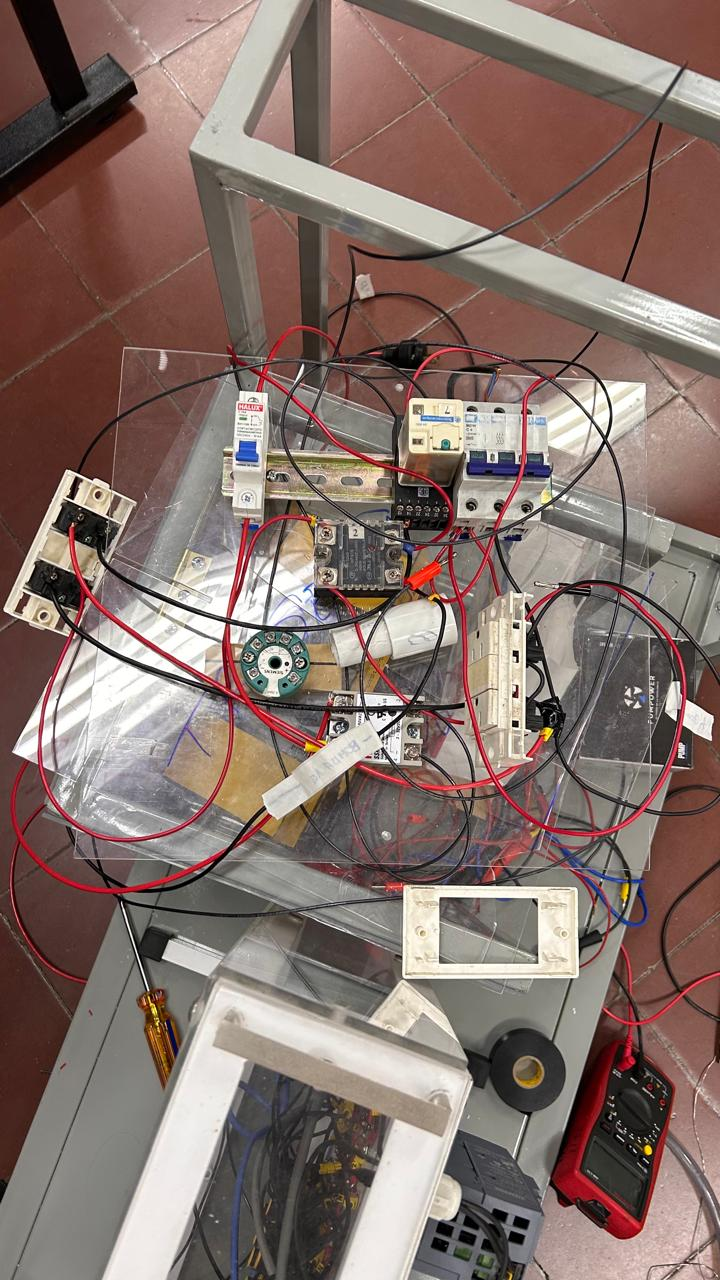
\includegraphics[width=0.4\textwidth]{archivos_complementarios/evidencias-fotograficas/montaje1-16oct-tablero.jpeg}
\caption{Conexionado y verificación del tablero de potencia durante las pruebas (16 de octubre de 2026).}
\label{fig:prueba_montaje_01}
\end{figure}

\subsection{Observaciones de seguridad derivadas del montaje}

Durante el montaje se identificaron cuatro aspectos de seguridad que se incorporaron a la matriz de riesgos:

\begin{itemize}
\item A la tensión medida de 126,3\,V, la resistencia de inmersión consume 16,2\,A medidos con pinza amperimétrica (2046\,W, Sección~\ref{sec:montaje_control}), un valor superior a la corriente nominal del interruptor automático de 15\,A que la protege.
\item Los SSR operan sin disipador adicional, solo con su placa metálica; el SSR de la resistencia disipa del orden de 20\,W a plena carga, por lo que su temperatura debe vigilarse durante los periodos largos de calentamiento.
\item Sin el termostato bimetálico, que no se adquirió en este corte por presupuesto, el único corte por sobretemperatura es el programado en el PLC al superar 40\,°C, de modo que una falla del SSR en cortocircuito no tendría un respaldo independiente.
\item La bomba de impulsión no cuenta con guardamotor, por lo que carece de protección térmica propia frente a sobrecarga.
\end{itemize}

Las acciones frente a estas observaciones están pendientes. Por ahora, la temperatura de los SSR se vigila durante los calentamientos, y la incorporación de un termostato bimetálico, que no se adquirió por presupuesto, está por decidir. Como acciones correctivas se recomiendan cambiar Q1 por un interruptor de 20\,A, después de verificar que el cableado del ramal sea al menos de calibre 12\,AWG; montar un disipador con pasta térmica en el SSR de la resistencia, e instalar un termostato bimetálico en serie con la resistencia como respaldo del corte por programa.

\subsection{Pruebas pendientes}

Quedan por completar las pruebas pendientes de la Tabla~\ref{tab:resultados_pruebas} (VAL-07 y VAL-08; la prueba de tinta, VAL-13, no se realizó) y las de aceptación que aún faltan: una prueba continua de 30\,min, tres valores de consigna dentro del rango seguro con una perturbación controlada, la comparación entre la respuesta experimental y la simulada, y la medición de la latencia y del porcentaje de registros recibidos (meta de al menos 99\,\%).